\documentclass[12pt]{article}
 
\newenvironment{sol}[1][Solution]{\begin{trivlist}\item[\hskip\labelsep {\bfseries #1:}]}{\end{trivlist}}
\usepackage{minted}
%\usemintedstyle{perldoc}
\usemintedstyle{vs}
\usepackage{graphicx}
\graphicspath{./}

\usepackage[margin=1in]{geometry} 
\usepackage{amsmath,amsthm,amssymb}
\usepackage{times,url}
\usepackage{tikz}
\usepackage{enumerate}
\begin{document}
\renewcommand{\qedsymbol}{\filledbox}
\begin{center}
    \textbf{CS 5/7350 - Test\#1} \\
    \textbf{March 17, 2021}
%replace X with the appropriate number
\end{center}
\begin{flushright}
Name: \underline{Bingying Liang }\\
ID:  \underline{\ \ \ \ \ 48999397 \ \ \ \ \ }
\end{flushright}

\begin{enumerate}
    \item \ [8 pts] You run different programs for various values of “n” and create 4 tables of the runtimes. Give the Asymptotic bounds that each of the tables support?
     \begin{center}
            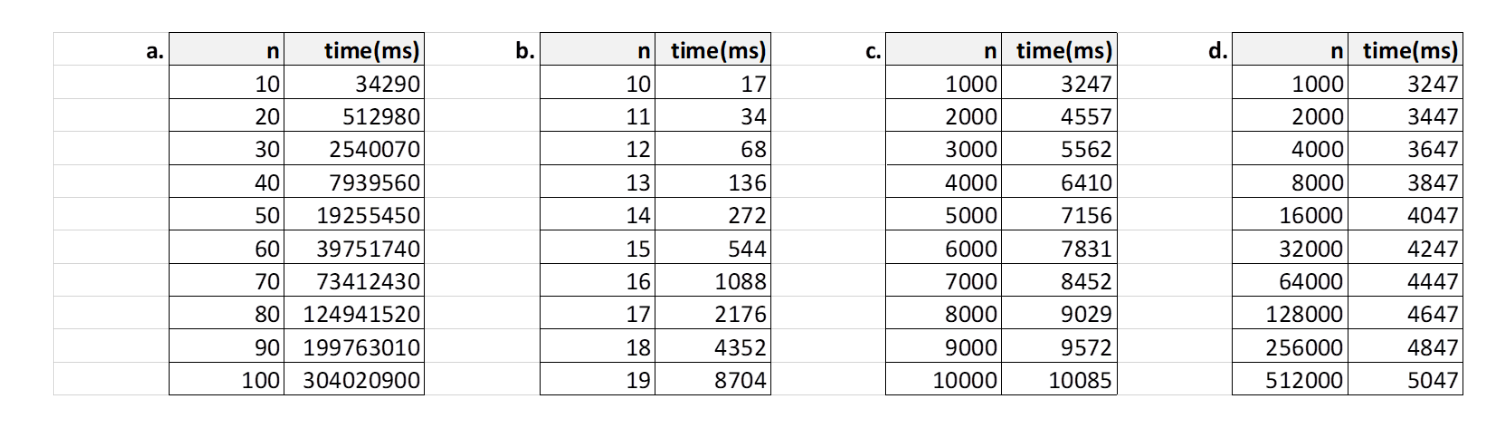
\includegraphics[width = 0.9\textwidth]{p1.png}
    \end{center}
    \begin{sol}
    \begin{enumerate}
        \item $\Theta(n^4)$
        \item $\Theta(2^n)$
        \item $\Theta(\sqrt{n})$
        \item $\Theta(\log(n))$
    \end{enumerate}
    \end{sol}

    \item \ [6 pts] Consider two different algorithms that each solve a different problem.
    \begin{itemize}
        \item Algorithm X solves Problem $P_x$ and Algorithm X is $\Theta(n_2)$
        \item Algorithm Y solves Problem $P_y$ and Algorithm Y is $\Theta(n_3)$
    \end{itemize}
    Determine if each of these “Yes it is true”, “Maybe it is true but doesn’t have to be”, or “No it is not true”
    \begin{enumerate}
        \item Problem $Px$ is easier than Problem $Py$: M
        \item Problem $Py$ is easier than Problem $Px$: M
        \item Algorithm X is easier than Algorithm Y: Y
        \item Algorithm X is $\Omega(n^2)$: Y
        \item Algorithm X is $\omega(n^2)$: N
        \item Algorithm Y is $\Omega(n^2)$: Y
    \end{enumerate}

    \item \ [5 pts] Given that $M > 100$ and $7_{31121} mod M = 9$ and $A = {1, 2, 3, 4}$ and $B = {A, B, C, D}$
    \begin{enumerate}
        \item $7^{31122} \bmod M = $  63
        \item $7^{62242} \bmod M = $ 81
        \item $\frac{1}{3} \bmod 11 = $ 4
        \item $|A\times B|$ = 16
        \item \textcolor{red}{$2^{125} \bmod 11$ = 10}
    \end{enumerate}

    \item \ [8 pts] How many bits of entropy are in the following messages?
        \begin{enumerate}
            \item A message that contains 20 H’s and 80 T’s?
            \begin{sol}
            72.19 bits
            \end{sol}

            \item A message that contains 30 H’s and 70 T’s?
            \begin{sol}
            88.129 bits
            \end{sol}

            \item A message that contains 0 H’s and 100 T’s?
            \begin{sol}
            0 bits
            \end{sol}

            \item A message that contains 50 H’s and 50 T’s?
            \begin{sol}
            100 bits
            \end{sol}

        \end{enumerate}

    \item \ [5 pts] Define Algorithm
    \begin{sol}
    A step by step procedure for solving a problem in a finite amount of time.
    \end{sol}

    \item \ [8 pts] A 100 character message containing only A, B, C and D’s is Huffman encoded. For each of the following codes, determine if they are valid. If they are not, explain why they are not and if they are valid, give a number of A, B, C and Ds that could generate that code:
    \begin{enumerate}
        \item A = 00; B = 01; C = 10; D = 11
        \begin{sol}
        Valid, A: 25, B: 25, C: 25, D: 25
        \end{sol}
        \item A = 1; B = 01; C = 00; D = 001 
        \begin{sol}
            Invalid, 001 could be ``CA" or ``D"
        \end{sol}
        \item A = 1; B = 01; C = 000; D = 001
        \begin{sol}
            Valid, A: 50, B: 30, C:10, D:10
        \end{sol}
        \item A = 1; B = 0; C = 10; D= 11
        \begin{sol}
        Invalid, 10 could be AB or C
        \end{sol}
    \end{enumerate}

    \item \ [6 pts] Argue that the problem, S, of sorting an unsorted array of integers is at least as hard as and possibly harder than the problem, H, of creating a MIN\_HEAP of that array.
    \begin{sol}
    Since the solution to the problem of sorting an array can be used for creating a Min-Heap (because a sorted array is a min-heap), Problem S must be just as hard or possible harder than problem H.
    \end{sol}

    \item \ \textcolor{red}{[6 pts] Draw all the non-isomorphic trees on 5 vertices.}
    \begin{sol}
             \begin{center}
            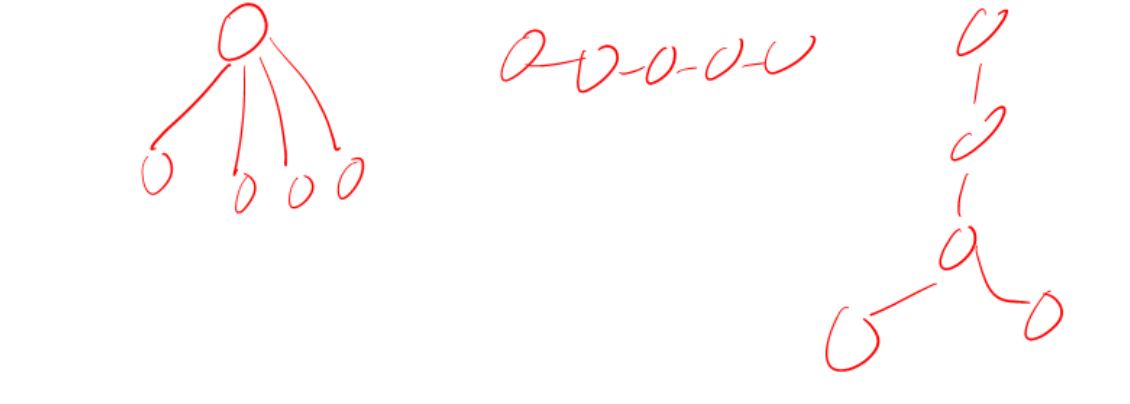
\includegraphics[width = 0.9\textwidth]{p2.png}
    \end{center}
    \end{sol}

    \item \ \textcolor{red}{[6 pts] We want to play a game called guess an integer “n”. I will think of an integer. You can offer guesses and I’ll tell you “higher” or “lower. Give an algorithm for guessing n that requires $\Theta(lg(n))$ guesses. (Hint, $\Theta(lg(n))$ could be $2 lg (n)$ or $3 lg(n)$ – To answer a common question, there is no upper bound, but the number of guesses is allowed to grow based on the size of the chosen number)}
    \begin{sol}
        \hspace*{\fill}\\
        Guess = 1\\
        While (ASK is Guess $<$ answer == yes) \{Guess = Guess * 2\} \\
        Binary search for answer between Guess and Guess/2
    \end{sol}

    \item \ \textcolor{red}{[6 pts] You are designing a Diffie-Hellman key exchange. You choose the base of 3. Would 7, 11 or 13 make a better modulus for that base? Why?}
    \begin{sol}
    7 is better since it cycles through more values before running to 1.
    \begin{align*}
        3^1 \bmod 7 = 3 \\
        3^2 \bmod 7 = 2 \\ 
        3^3 \bmod 7 = 6 \\ 
        3^4 \bmod 7 = 4 \\
        3^5 \bmod 7 = 5 \\ 
        3^6 \bmod 7 = 1 \\
        3^7 \bmod 7 = 3 \\
        \\        
        3^1 \bmod 11 = 3 \\
        3^2 \bmod 11 = 9 \\ 
        3^3 \bmod 11 = 5 \\ 
        3^4 \bmod 11 = 4 \\
        3^5 \bmod 11 = 1 \\ 
        3^6 \bmod 11 = 3 \\
        \\
        3^1 \bmod 13 = 3 \\
        3^2 \bmod 13 = 9 \\ 
        3^3 \bmod 13 = 1 \\ 
        3^4 \bmod 13 = 3 \\
    \end{align*}
    \end{sol}

    \item \ \textcolor{red}{[7 pts] Consider performing a Breath First Search of the following graph starting at S. Give the order the vertices are popped from the queue:}
                 \begin{center}
            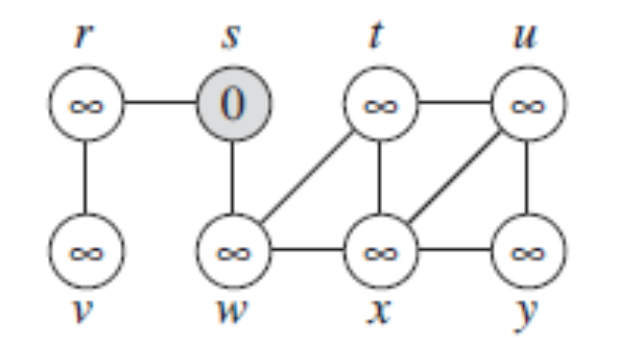
\includegraphics[width = 0.4\textwidth]{p3.png}
    \end{center}
    \begin{sol}
    SRWVTXUY
    \end{sol}

    \item \ [7 pts] Give the discover and finalize time for each vertex of the following graph when performing a Depth First Search starting at U.
                             \begin{center}
            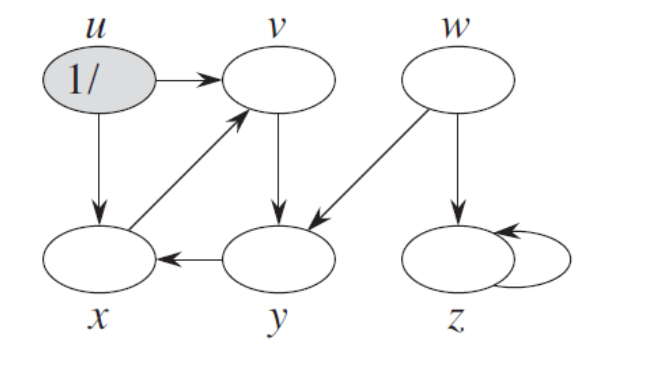
\includegraphics[width = 0.4\textwidth]{p4.png}
    \end{center}
    \begin{sol}
    \hspace*{\fill}\\
                         \begin{center}
            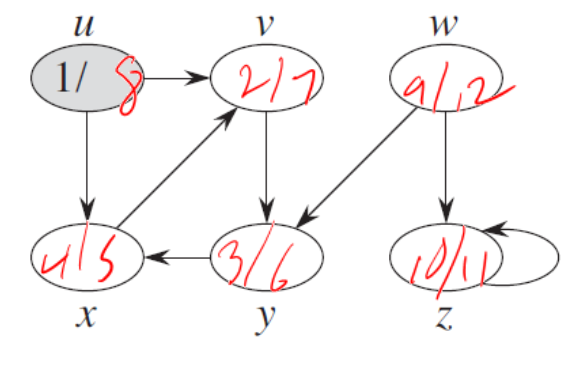
\includegraphics[width = 0.4\textwidth]{p5.png}
    \end{center}
    \end{sol}

    \item \ \textcolor{red}{[8 pts] Consider the following graph. For any questions needing a starting vertex, use vertex S as the starting vertex.}
                             \begin{center}
            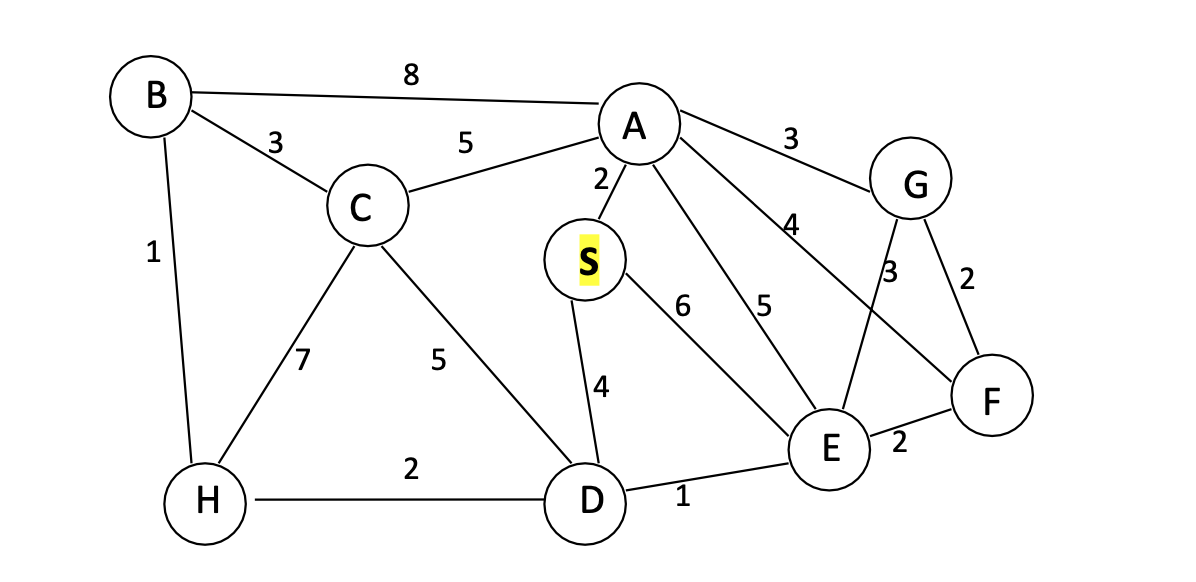
\includegraphics[width = 0.9\textwidth]{p6.png}
    \end{center}
    \begin{enumerate}
        \item What is the value of the third edge chosen when finding a minimum spanning tree using Prim's algorithm?
        \begin{sol}
            2
        \end{sol}
        \item What is the value of the third edge chosen when finding a minimum spanning tree using Kruskal's algorithm?
        \begin{sol}
        2
        \end{sol}
        \item When using Dijkstra's algorithm to find the shortest path from S to all vertices, what is the order in which the vertices are reached?
        \begin{sol}
        S A D E G F H B C 
        \end{sol}

        \item What is the weight of the minimum spanning tree?
        \begin{sol}
        16
        \end{sol}
    \end{enumerate}
    \item  [8 pts] The graph below represents containers that are transported between these cities each day. You are determining the maximum flow from vertex S, Vancouver, to vertex T, Winnipeg, using the Ford-Fulkerson algorithm in the graph below. A Breadth First Search finds the path $s \rightarrow v_1 \rightarrow v_3 \rightarrow v_2 \rightarrow v_4 \rightarrow t$. What does the new graph look like after “removing” this flow?
        \begin{center}
            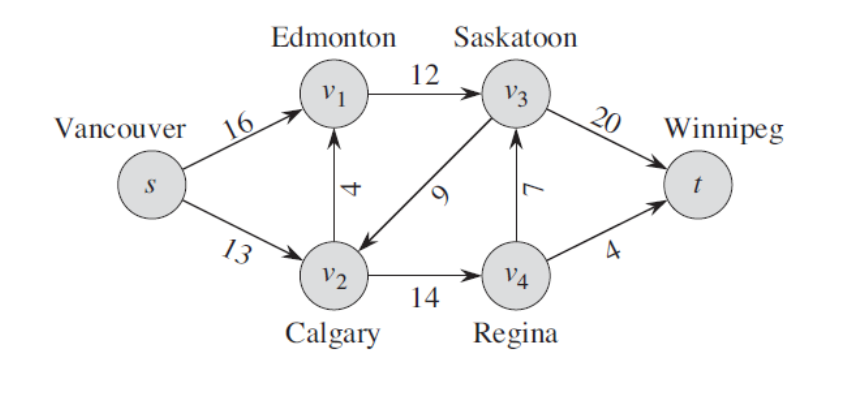
\includegraphics[width = 0.6\textwidth]{p7.png}
    \end{center}
    \begin{sol}
    \hspace*{\fill}\\
        \begin{center}
            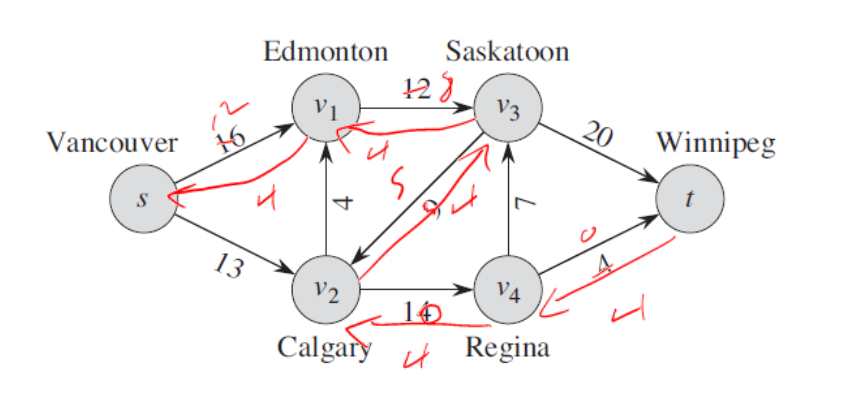
\includegraphics[width = 0.6\textwidth]{p8.png}
    \end{center}
    \end{sol}

    \item \ [6 pts] A particular algorithm on a computer requires 2 seconds to process $200$ items and is $\Theta(n^3)$. You want to process $4000$ items. You have a choice to either use a computer that is $10$ times faster (allowing it to process $200$ items in $0.2$ seconds) or use the same computer with a different algorithm that still processes $200$ items in $2$ seconds, but has a growth rate that is $\Theta(n^2)$.
    \begin{enumerate}
        \item Which is the faster choice for $4000$ items?
            \begin{sol}
            Different algorithm
    \end{sol}
        \item For what input sizes is the faster computer better?
        \begin{sol}
        size $<2000$
        \end{sol}
        \item For what input sizes is the $\Theta(n^2)$ algorithm better?
        \begin{sol}
                size $> 2000$
        \end{sol}
    \end{enumerate}

\end{enumerate}
\end{document}
